\section{Entwicklung einer cross-kompilierten Applikation mit Flutter}
Der dritte Ansatz ist eine cross-kompilierte Umsetzung. Dabei wurde das Flutter Framework gewählt, da es laut einer aktuellen Statistik \cite{statist_CP_Framework} das meist genutzte Framework unter den Cross-Plattform Frameworks ist.

\subsection{Grundlagen}
\label{cha:4_3_1}
Flutter ist ein 2017 von Google veröffentlichtes Framework das mittlerweile zum meistgenutzten Cross-Plattform-Framework geworden ist \cite{statist_CP_Framework}. Die Popularität von Flutter ist beispielsweise auch in der Ankündigung der Firma Canonical\footnote{https://canonical.com/ - Entwicklerfirma hinter Ubuntu} zu erkennen, dass alle von ihnen entwickelten Ubuntu Desktop-Anwendungen, zukünftig mit Flutter entwickelt werden\cite{Ubuntu_Flutter}. Als Programmiersprache verwendet Flutter Dart. Der Code wird dabei je nach Plattform, mit einem speziellen Compiler in nativen Code übersetzt wird\cite{flutter_compilation}.

Alle gezeigten Komponenten einer Flutter App sind sogenannte Widgets. Neben den tatsächlich angezeigten Elementen der Benutzeroberfläche, können auch Gestenerkennung, Layouthelfer oder Logik als ein Widget eingebunden werden \cite{Thiele_2018}. Dabei werden Widgets baumartig verschachtelt. So können die meisten Widgets wieder ein oder mehr Kinderelemente der Klasse Widget besitzen. In Abbildung \ref{fig:flutter_layout_tree} ist der Widget-Baum einer Menüleiste zu sehen. Ein Container ist ein Dummy-Element, das wiederum ein anderes Widget enthält und etwa einen Abstand zu anderen Elementen definiert. Ein Container entspricht somit dem div-Element von HTML. Es gibt auch Widgets, die keine Kinder haben und bei denen der Baum endet. So etwa die in Abbildung \ref{fig:flutter_layout_tree} abgebildeten Text- und Icon-Widgets.

\begin{figure}[ht]
  \centering
  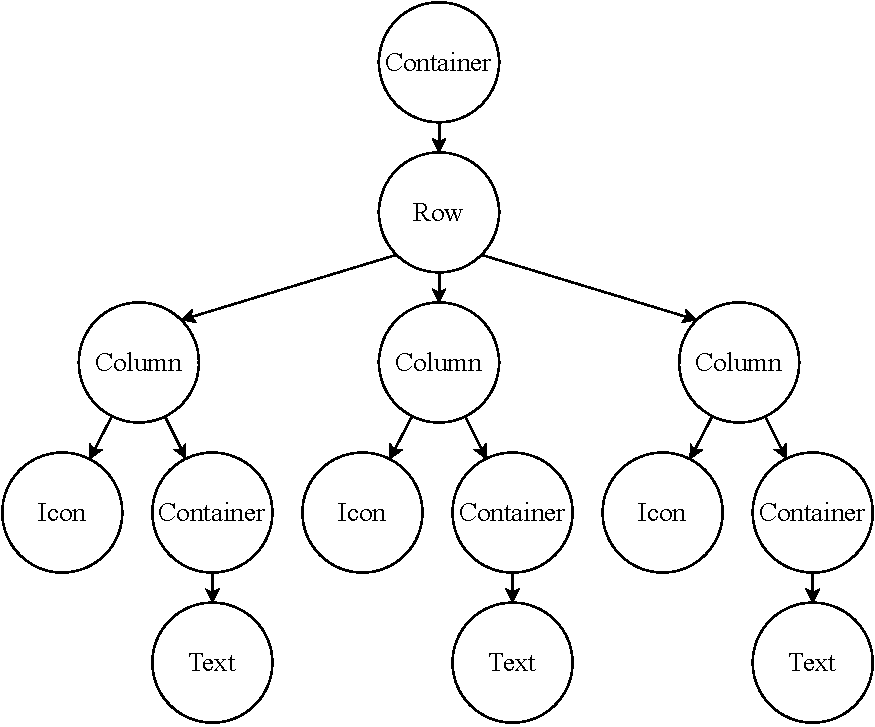
\includegraphics[height=8cm,keepaspectratio]{images/Flutter_menu_replacement.drawio.pdf} 
  \caption[Hierarchie einer Menüleiste]{Hierarchie einer Menüleiste - In Anlehnung an Flutter Dokumentation\protect\footnotemark}
  \label{fig:flutter_layout_tree}
\end{figure}

\footnotetext{https://docs.flutter.dev/development/ui/layout}

Anders als bei der nativen Implementierung werden bei Flutter Benutzeroberfläche und Funktionalität in Dart Code zusammen implementiert. So wird etwa die Funktionalität eines Knopfes, direkt bei der Deklaration diesem zugeordnet. Dafür muss das Widget in den Baum eingefügt werden und danach die Funktionalität in einem Attribut des Widgets eingestellt werden.

Da Flutter einen großen wert auf Performance legt, werden bei einer Änderung an der Oberfläche nur die betroffenen Elemente neu gebaut. Widgets die dieses dynamische Neubauen unterstützen, sind vom Typ \verb|StatefulWidget| und verwalten zusätzlich ein State-Objekt, welches ihren aktuellen Zustand repräsentiert \cite[Kapitel~4]{Flutter_Recipes}. Bei einer Änderung des Zustandes, registriert Flutter die Änderung und baut daraufhin das geänderte Widget und die daraus folgende Hierarchie neu\cite{9623025}. Dadurch kann häufiges und vor allem vollständiges Neubauen des Widget-Baums verhindert werden. Jedoch benötigt nicht jedes Element einen State. Wenn etwa bereits zum Zeitpunkt des Erzeugens des Widgets, alle Daten feststehen und unveränderbar sind, dann wird kein State benötigt und es reicht ein \verb|StatelessWidget| für die Implementierung \cite[Kapitel~4]{Flutter_Recipes}. Dadurch wird einerseits die Implementierung eines States ersparrt und bei einem Neubau des Baums, kann das Widget einfach wieder genutzt werden. Daher muss es lediglich neu gerendert werden.

Um Codewiederholung zu vermeiden, können in Flutter ein eigenes Widget erstellt werden. 
Diese können im gesamten Projekt, wie von Flutter bereitgestellte Widgets, in den Widget-Baum eingefügt werden. 
%Das Erstellen eines Widgets ist dabei der selbe Prozess wie das erstellen einer Seite. Es wird ein Knoten Element gewählt und dann mit anderen Elementen kombiniert, um die gewünschte Oberfläche zu erhalten. 
Dabei muss jedoch entschieden werden, ob es sich um ein \verb|Stateful-| oder \verb|StatelessWidget| handelt. Falls notwendig muss dann der benötigte State implementiert werden.


\subsection{Benutzte Packages}
\label{cha:4_3_2}
In Flutter gibt es für Erweiterungen ein zentrales Verzeichnis\footnote{https://pub.dev/}t, in dem alle verfügbaren Packages gefunden werden können. Hier können die verfügbaren Packages verglichen und eine Anleitung gefunden werden. Im Folgenden werden die verschiedenen genutzten Erweiterungen vorgestellt.

Ein wichtiges Package bei der Umsetzung der Applikation, ist \verb|graphql\_flutter|\footnote{https://pub.dev/packages/graphql\_flutter}. 
Dies stellt, ähnlich wie die in Kapitel \ref{cha:4_1_bibliothek} vorgestellte GraphQL-Bibliothek, einen Clienten für die Kommunikation mit der GraphQL Schnittstelle des Servers zur Verfügung.
Damit der Client von allen Seiten und Widgets benutzt werden kann, muss das GraphQL-Widget als Wurzel der Applikation gesetzt werden. Danach können, entweder über ein Widget oder über eine programmierte Funktion, die verschiedenen GraphQL Funktionen ausgeführt werden. 
Im Gegensatz zu der in der nativen genutzten Erweiterung wird jedoch die Antwort nicht automatisch konvertiert. So muss auf die einzelnen Felder der JSON-Antwort mit Hilfe der Klammern-Notation\footnote{\url{https://developer.mozilla.org/de/docs/Learn/JavaScript/Objects/Basics\#klammer-notation}} zugegriffen werden, wodurch die Gefahr eines fehlerhaften Zugriffs erhöht wird.

Ein weiteres wichtiges Package ist Hive\footnote{\url{https://pub.dev/packages/hive}}. Dieses stellt einen einfachen und schnellen Key-Value Speicher zur Verfügung. Dieser ermöglicht es Daten innerhalb der Applikation zu speichern und kann sie somit auch nach dem Neustart der App wieder zur Verfügung stellen. Im Rahmen dieser Arbeit wird dieser benutzt um den Identifikationsstring für den Server zu speichern. Es ist vergleichbar mit den \verb|SharedPreferences| aus der nativen Entwicklung. Zusätzlich ermöglicht Hive jedoch die Nutzung komplexeren Datentypen wie ganzer Listen oder die Verschlüsselung der gespeicherten Daten. Dabei werden Daten zwar etwas langsamer gelesen als in der nativen Implementierung, allerdings ist das Schreiben und Löschen von Daten deutlich schneller \cite{hive_vs_sharedPrefernces}.

Als dritte Erweiterung soll \verb|simple_gradient_text|\footnote{\url{https://pub.dev/packages/simple\_gradient\_text}} erwähnt werden. Dieses dient dazu, Farbverläufe auf Texte anzuwenden. Bei der Verwendung des Plugins wurden die Vorteile einer aktiven Entwicklergemeinschaft festgestellt. So gab es nach der Installation anfänglich das Problem, dass lediglich die Android Umsetzung funktionierte, obwohl alle Plattformen als unterstützt markiert waren. Bei der Kommunikation mit den Entwicklern des Plugins wurde klar, dass das Problem aufgrund einer zu geringen Dart-Version auftrat. Dies konnte durch eine kleine Anpassung behoben werden und die Funtkionalität des Plugins genutzt werden. Abschließend wurde die Dokumentation des Plugins auf GitHub und im zentralen Package-Verzeichnis angepasst.

Zuletzt soll das Package \verb|sqflite_common_ffi|\footnote{\url{https://pub.dev/packages/sqflite\_common\_ffi}} erwähnt werden, welches für die Bereitstellung einer Datenbank genutzt wurde. Dieses bietet auf Basis von \verb|SQLite3|\footnote{\url{https://www.sqlite.org/}} eine Datenbankimplementierung für alle Plattformen an.
Die Datenbank wird beim Start der Anwendung gestartet und steht anschließend als globales Attribut der gesamten Anwendung zur Verfügung.
Die Benutzung ist dabei recht simpel, da zur Erstellung einer Tabelle lediglich der entsprechende SQL-Befehl ausgeführt werden muss.
Danach kann über dedizierte Einfüge und Abfrage Methoden die Daten gespeichert beziehungsweise abgefragt werden.
Zusätzlich können auch selbst formulierte SQL-Befehle ausgeführt werden. So können alle im SQL-Standard enthaltenen Funktionalitäten genutzt werden.


\subsection{Exkurs: Platform spezifische Funktionalität entwickeln}
Im Verlaufe der Entwicklung kann es vorkommen, dass Plattform-Funktionalität genutzt werden soll und kein entsprechendes Plugin existiert.
Für diesen Fall ermöglicht Flutter die Programmierung eines eigenen Plugins.
Für diesen Fall kann ein eigenes Plugin geschrieben werden. 
Der Aufbau eines solchen Plugins kann schematisch in Abbildung \ref{fig:flutter_plattform_specific} gesehen werden. 
Einerseits wird der Dart-Code benötigt, welcher die Funktionalität des Plugin definiert und die Daten wenn benötigt weiterverarbeitet. 
Zusätzlich wird der Plattform Code für die erwünschten Plattformen benötigt. Dieser realisiert die Funktionalität in einer nativen Implementierung.
Zur Kommunikation wird der sogenannte MethodChannel verwendet. Dieser erlaubt einen bidirektionale Datenaustausch zwischen den plattform-unabghängigen und den plattform-spezifischen Codeanteilen \cite[Kapitel~12.3]{Flutter_Recipes}.

\begin{figure}[ht]
  \centering
  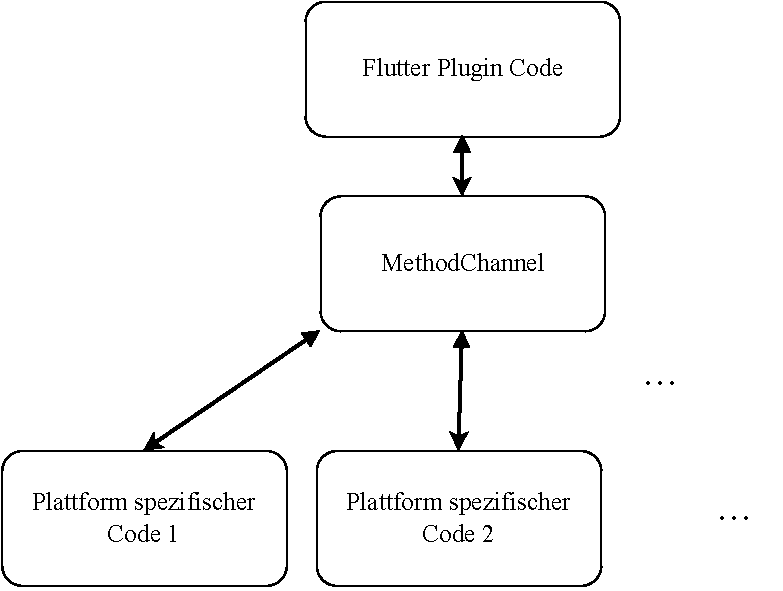
\includegraphics[width=9cm,keepaspectratio]{images/flutter_plattform_specific.pdf} 
  \caption[Aufbau eines Plugins mit plattformspezifischen Code]{Aufbau eines Plugins mit plattformspezifischen Code - in Ahnlehnung an Flutter Dokumentation\protect\footnotemark}
  \label{fig:flutter_plattform_specific}
\end{figure}

\footnotetext{\url{https://docs.flutter.dev/resources/architectural-overview}}

Durch die Nutzung von Kommunikationskanälen wird die parallele Ausführung des Plattform Codes in einem separaten Thread ermöglicht. Dieser kann asynchron ausgeführt werden und blockiert somit nicht den Thread, welcher die graphische Oberfläche verwaltet. Dadurch kann dieser weiterhin auf Eingaben durch den Nutzer reagieren \cite{plattform_code_flutter}.

Es ist folglich möglich, benötigte Funktionalität hinzuzufügen, solange sie auf den einzelnen Plattformen umsetzbar ist. Da dafür jedoch plattform-spezifische Implementierungen notwendig sind, muss der Entwickler fähig ein, den Code für jede Plattform umzusetzen.

\subsection{Exkurs: Firebase}
Ein weiterer Grund für die Nutzung von Flutter bei keineren App-Projekten, ist die Möglichkeit der einfachen und umfangreichen Integration von Firebase\footnote{\url{https://firebase.google.com/}}. Eine Untersuchung \cite{statist_analytics_SDK} ergab, dass 92\% aller Android Applikationen, die eine Analyse Software integriert haben, Firebase nutzen.

Firebase ist eine Backend-as-a-service Lösung, welche sowohl die Entwicklung und den Betrieb von Anwendungen vereinfachen und beschleunigen soll. Firebase stellt eine Sammlung von verschiedensten Tools und Plugins bereit. Somit können Entwickler sich auf Design und Funktionalität der App konzentrieren. Eines dieser Tools ist das oben erwähnte Anaöyse-Tool zum Erstellen und Analysieren von Nutzungsdaten. Weiterhin stellt Firebase auch ein fertiges Chatsystem oder auch eine Cloud-Datenbank zur Verfügung. Guzzi et Al \cite{Flutter_Apprentice} betonen, dass das eigenständige Erstellen eines solchen Backends mehrere Monate dauern kann und somit nicht nur die Fertigstellung verzögert, sondern auch die Kosten der Applikation erhöht. Ein bereits bestehendes System wie Firebase, kann einen Anteil dieses Aufwandes übernehmen. Weiter stellen sie fest, dass dadurch tausende Zeilen Code eingesparrt werden können. Außerdem bietet Firebase die Möglichkeit asynchrone Aufrufe und nebenläufige Prozesse zu nutzen und somit die Reaktionsfähigkeit der App zu verbessern.

Ein großer Vorteil von Firebase ist die Entwicklungsgeschwindigkeit. So können Backend-Komponenten schnell erstellt und eingebunden werden. Um  etwa eine Datenbank zu erstellen sind gerade einmal wenige Schritte nötig. Nach dem Erzeugen der Datenbank auf der Firebase-Webseite, können die erzeugten Konfigurationsdateien heruntergeladen und in die Flutter-App eingefügt werden. Abschließend müssen nur noch die benötigten Datenstrukturen in der Applikation definiert werden. Danach kann über die in der Konfigurationsdatei definierte Schnittstelle mit dem Backend kommuniziert werden. Dazu kommt, dass neben einer online Datenbank, ebenfalls eine offline Version aktiviert werden kann. Diese wird dabei automatisch synchronisiert, sobald aktive Internetverbindung zur Verfügung steht \cite{flutter_firebase}.

Ein weiterer wichtiger Service, dem Firebase anbietet, ist die Firebase-Authentifizierung\footnote{\url{https://firebase.google.com/docs/auth}}. Diese bietet bietet eine fertige Lösung zur Authentifizierung von Nutzern. Weiterhin können Nutzer organisiert werden und Zugriffsbeschränkungen für bestimmte Nutzer umgesetzt werden. Beispielsweise kann mittels Regeln, präzise definiert werden, welche Nutzer auf welche Daten zugreifen können. Somit stellt die Firebase-Authentifizierung eine vielseitige und umfangreiche Identitäts- und Zugriffsmangament Lösung dar \cite{Flutter_Apprentice}.

Firebase kann nicht exklusiv mittels Flutter genutzt werden. So können genauso die verschiedensten Programmiersprachen der Plattformen Firebase einbinden. 
Dennoch ergibt sich bei der Kombination von Flutter und Firebase ein interessantes Gesamtsystem.
So kann durch Flutter die Schnittstellen zu Firebase leidlich einmal umgesetzt werden anstatt dies für jede Plattform einzeln machen zu müssen.
Dabei wird nicht nur Entwicklungsarbeit eingespart, sondern auch eine unterschiedliche Definition von Datenentitäten verhindert.


\subsection{Fazit cross-kompilierte Applikation}
Durch die hier beschriebene Entwicklung, kann mit nur einer einzelnen Code-Basis eine Anwendung geschrieben werden, die sowohl auf Android, iOS, Windows, Mac und Linux läuft. Lediglich bei der Web-Version trat ein Problem mit dem GraphQL-Client auf, da dieser in der Web-Version keine Verbindung erstellen konnte. Für alle anderen Plattformen musste lediglich die Unterstützung in der Konfigurationsdatei von Flutter deklariert, der Code in plattformspezifischen Code kompiliert und ausgeführt werden.

Der Entwicklungsaufwand einer Flutter Applikation ist dabei mit der Entwicklung einer nativen Applikation für lediglich eine Plattform vergleichbar. Dabei entsteht jedoch Implementierungen für alle von Flutter unterstützten Plattformen zugleich. Selbst wenn der Fokus der Entwicklung zuerst nur auf einer Plattform liegt, kann es somit sinnvoll sein Flutter zu nutzen, um in Zukunft ohne großen Aufwand weitere Plattformen hinzuzufügen.
Dabei muss jedoch auf mögliche Kompatibilitätsprobleme geachtet werden. So entstand bei der vorgestellten Implementierung keine funktionierende Web-Version, da diese mit dem genutzten GraphQL-Package inkompatibel war.
Dies sollte bei der Wahl der Erweiterungen bedacht werden, um eine Inkompatibilität mit den gewünschten Plattformen zu umgehen. 
Wie bereits ausgeführt, können solche Probleme durch eine eigene Implementierung gelöst werden, dies ist jedoch mit einem erhöhten Aufwand und nötigen Plattform-Wissen verbunden.

Flutter ist außerdem ein noch recht neues Framework, daher werden regelmäßige Updates mit größere Änderungen eingeführt, die die Qualität und Entwicklung verbessern. Jedoch kann dabei auch eine umfangreiche Änderungen in der Implementierung notwendig werden. So wurde etwa ein Update veröffentlicht, dass die Null-Safety verbessert hat. In Folge dessen musste allerdings jede Bibliothek angepasst sowie viele der bestehenden Applikationen angepasst werden.